% !TeX root = ../main.tex

\begin{frame}
  \frametitle{{\small Coverage Testing for {\color{red} Topological Scalar Field Analysis}}}

  \begin{textblock*}{12cm}(1cm,2cm)
    Sample $P\subset D$ of $f : D\to \R$.\vspace{1ex}

    \only<2>{Cover $P^\delta = \bigcup_{p\in P}\ball^\delta(p)$.\vspace{1ex}}

    \only<3>{Analyze with discrete representation.}

  \end{textblock*}

  \begin{textblock*}{12cm}(1cm,5cm)
    \includegraphics<1>[trim=200 600 200 800, clip, width=0.5\textwidth]{figures/partial3/samples}
    \includegraphics<2>[trim=200 600 200 800, clip, width=0.5\textwidth]{figures/partial3/cover}
    \includegraphics<3>[trim=200 600 200 800, clip, width=0.5\textwidth]{figures/partial3/complex}
    % \includegraphics<3>[trim=200 600 200 800, clip, width=0.5\textwidth]{figures/samples/complex1}
  \end{textblock*}
\end{frame}

\begin{frame}
  \frametitle{Simplicial Complexes}

  \begin{textblock*}{11cm}(1cm,2cm)
    \begin{small}
      \only<1,2>{Vertex set $V$.\vspace{1ex}

      An (abstract) \emph{$k$-simplex} is a collection of $k+1$ vertices.\vspace{1ex}}

      \only<2>{A \emph{simplicial complex} $K$ is a collection of simplices that is closed under taking subsets.\vspace{1ex}}

      \only<3,4>{The \emph{boundary} of a $k$-simplex is a $(k-1)$ cycle.\vspace{1ex}}

      \only<4>{A $k$-cycle in $K$ has non-trivial homology if it is not the boundary of a $(k+1)$-\emph{chain}.}
    \end{small}
  \end{textblock*}

  \begin{textblock*}{11cm}(1cm,4.5cm)
    \includegraphics<1,2>[trim=0 0 -400 0, clip, width=0.3\textwidth]{figures/edge}
    \includegraphics<1,2>[trim=0 0 -200 0, clip, width=0.3\textwidth]{figures/tri}
    \includegraphics<1,2>[trim=-200 0 0 0, clip, width=0.3\textwidth]{figures/tet}
    \includegraphics<3,4>[trim=0 0 -400 0, clip, width=0.3\textwidth]{figures/edge_bdy}
    \includegraphics<3,4>[trim=0 0 -200 0, clip, width=0.3\textwidth]{figures/tri_loop}
    \includegraphics<3,4>[trim=-200 0 0 0, clip, width=0.3\textwidth]{figures/tet_void}
  \end{textblock*}
\end{frame}

% \begin{frame}
%   \frametitle{Homology of Simplicial Complexes}
%
%   \begin{textblock*}{11cm}(1cm,2cm)
%     \begin{small}
%       The \emph{boundary} of a $k$-simplex is a $(k-1)$ cycle.\vspace{1ex}
%
%       \only<2>{A $k$-cycle in has non-trivial homology if it is not the boundary of a $(k+1)$-\emph{chain}.}
%     \end{small}
%   \end{textblock*}
%
%   \begin{textblock*}{11cm}(1cm,4.5cm)
%     
\includegraphics[trim=0 0 -400 0, clip, width=0.3\textwidth]{figures/edge_bdy}
%     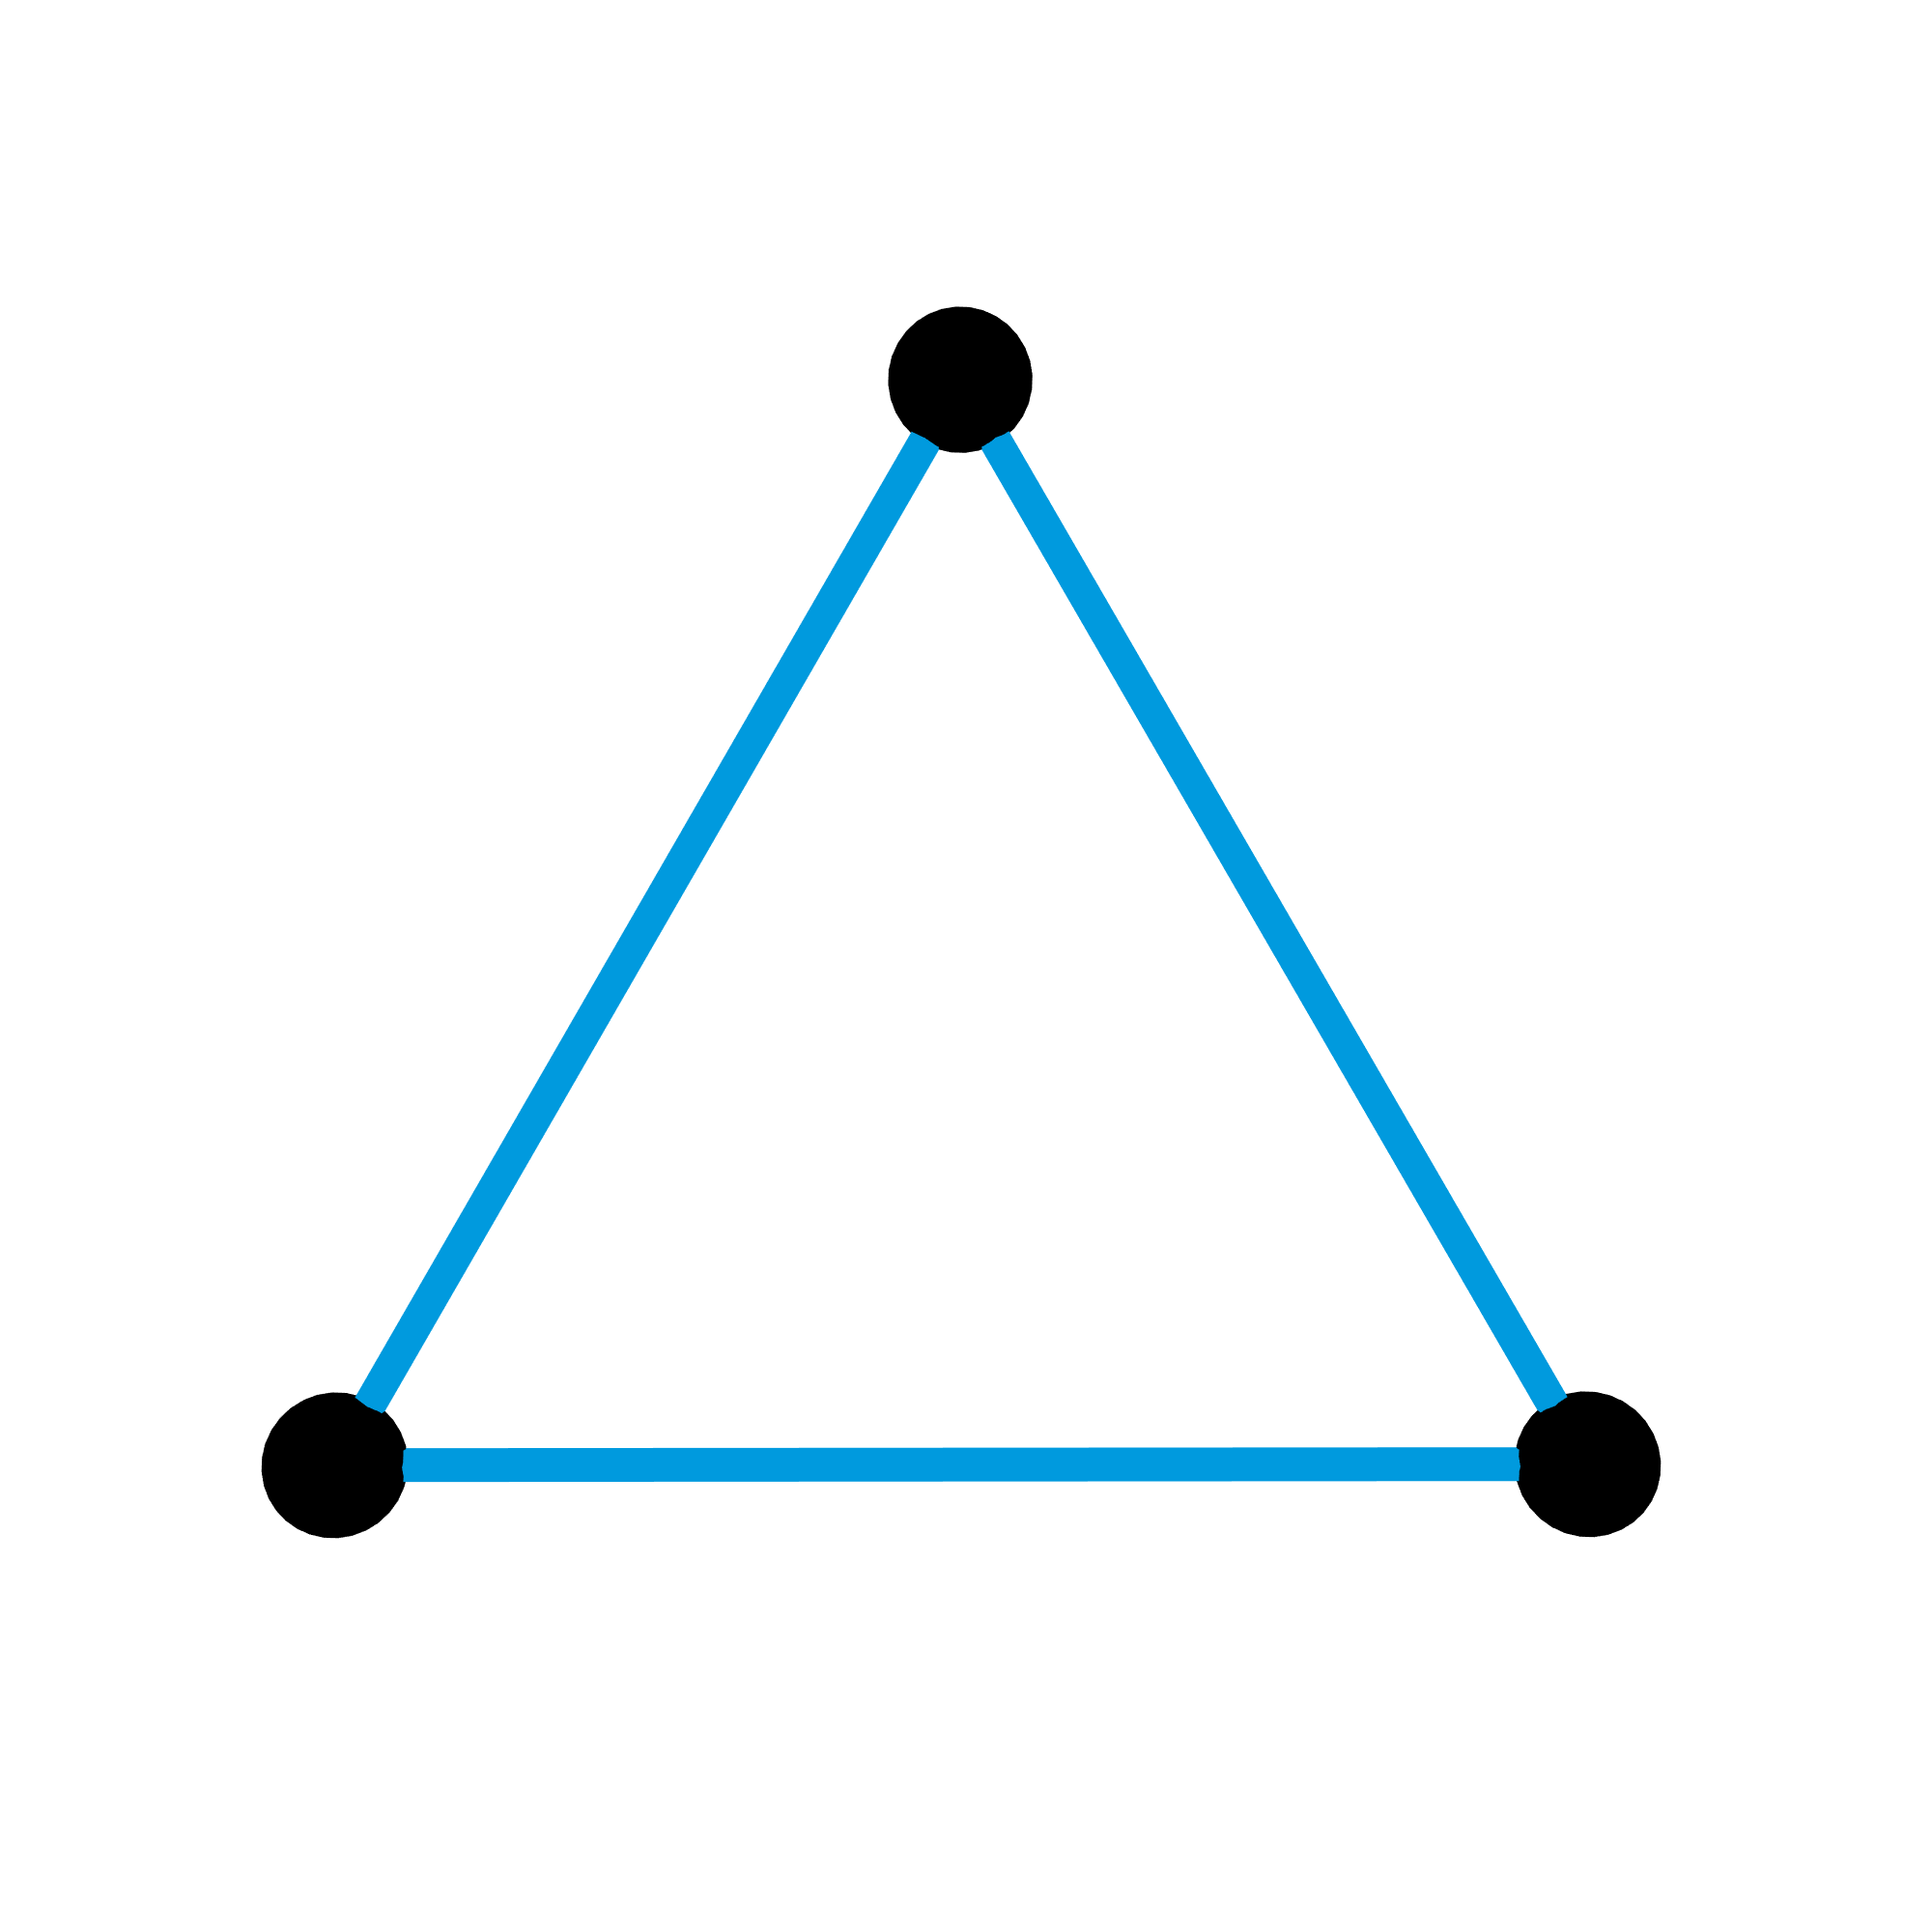
\includegraphics[trim=0 0 -200 0, clip, width=0.3\textwidth]{figures/tri_loop}
%     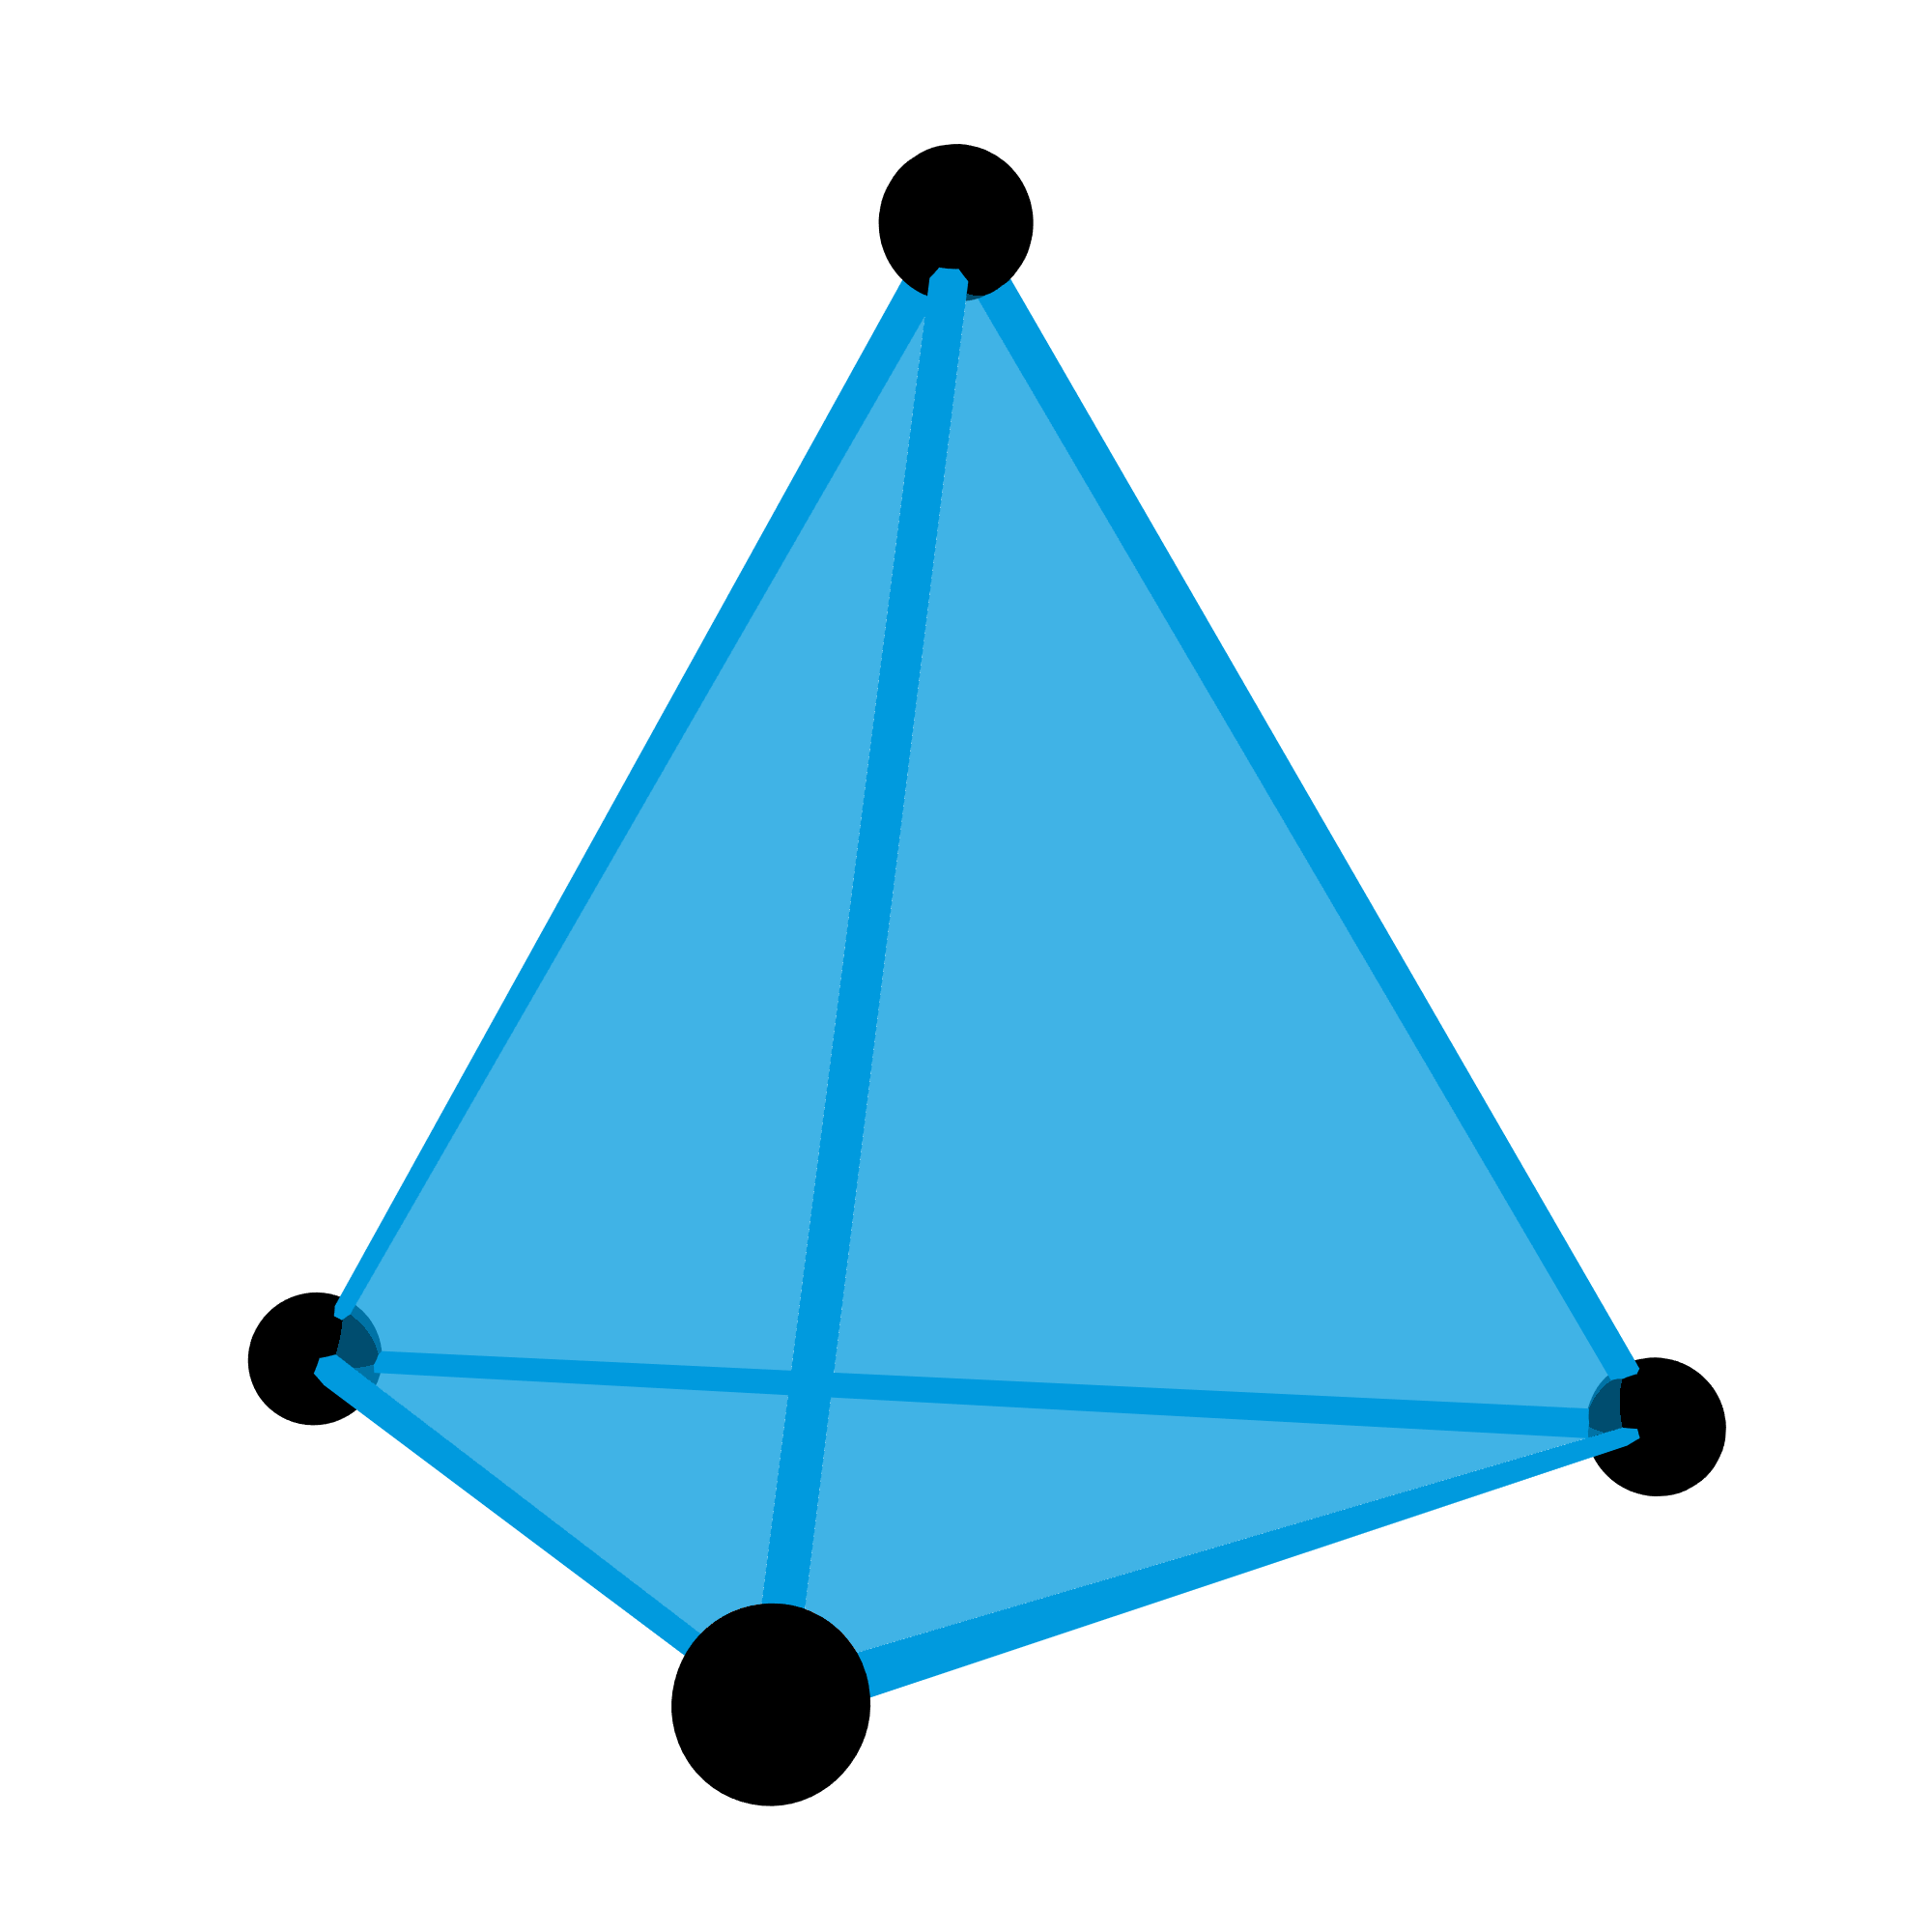
\includegraphics[trim=-200 0 0 0, clip, width=0.3\textwidth]{figures/tet_void}
%   \end{textblock*}
% \end{frame}

% \begin{frame}
%   \frametitle{The Clique Complex}
%
%   \begin{textblock*}{11cm}(1cm,2cm)
%     \begin{small}
%       \only<1,2>{Graph $G$.\vspace{1ex}}
%
%       \only<2>{The \emph{clique complex} of $G$ has a $(k-1)$-simplex for each $k$-clique.\vspace{1ex}}
%     \end{small}
%   \end{textblock*}
%
%   \begin{textblock*}{12cm}(1cm,4.5cm)
%     \includegraphics<1>[trim=50 400 75 500, clip, width=0.5\textwidth]{figures/rips/graph_nocov}
%     \includegraphics<2>[trim=50 400 75 500, clip, width=0.5\textwidth]{figures/rips/clique}
%   \end{textblock*}
%
% \end{frame}
%
% \begin{frame}
%   \frametitle{Nerves of Covers}
%
%   \begin{textblock*}{11cm}(1cm,2cm)
%     \begin{small}
%       \only<1,2,3,4>{A collection $\U = \{U_i\}_{i\in I}$ is a \emph{cover} of $D$ if $\bigcup_{i\in I} U_i = D$.\vspace{2ex}}
%
%       \only<2,3,4>{The \emph{nerve} of $\U$ has a $(k-1)$-simplex for each $k$-wise intersection.}
%
%       \only<5>{The \emph{Nerve Theorem} states that the nerve of a \emph{good} open cover captures the homology of its union.}
%     \end{small}
%   \end{textblock*}
%
%   \begin{textblock*}{12cm}(1cm,4.5cm)
%     \includegraphics<1>[trim=50 400 75 500, clip, width=0.5\textwidth]{figures/nerves/cover}
%     \includegraphics<2>[trim=50 400 75 500, clip, width=0.5\textwidth]{figures/nerves/cover-points}
%     \includegraphics<3>[trim=50 400 75 500, clip, width=0.5\textwidth]{figures/nerves/two-edges-points}
%     \includegraphics<4>[trim=50 400 75 500, clip, width=0.5\textwidth]{figures/nerves/three-tri}
%     \includegraphics<5>[trim=50 400 75 500, clip, width=0.5\textwidth]{figures/nerves/full}
%   \end{textblock*}
% \end{frame}

\begin{frame}
  \frametitle{The \v Cech Complex}

  \begin{textblock*}{11cm}(1cm,2cm)
    \begin{small}
      \only<1-6>{Finite $P\subset D$.\vspace{1ex}}

      \only<2-6>{Cover $\{\ball^\delta(p)\}_{p\in P}$ of open metric balls.\vspace{1ex}}

      \only<3-6>{The \emph{\v Cech complex} $\cech^\delta(P)$ has a $(k-1)$-simplex for each $k$-wise intersection.\vspace{1ex}}

      % \only<3>{The nerve of this cover is the \emph{\v Cech complex} $\cech^\delta(P)$.}

      \only<7>{The Nerve Theorem: \[\hom_k(\cech^\delta(P))\cong\hom_k(P^\delta).\]}
    \end{small}
  \end{textblock*}

  \begin{textblock*}{12cm}(1cm,4.5cm)
    \includegraphics<1>[trim=50 400 75 500, clip, width=0.5\textwidth]{figures/cech2/points}
    \includegraphics<2>[trim=50 400 75 500, clip, width=0.5\textwidth]{figures/cech2/cover}
    \includegraphics<3>[trim=50 400 75 500, clip, width=0.5\textwidth]{figures/cech2/full}
    \includegraphics<4>[trim=50 400 75 500, clip, width=0.5\textwidth]{figures/cech2/inter2-edge}
    \includegraphics<5>[trim=50 400 75 500, clip, width=0.5\textwidth]{figures/cech2/inter3-tri}
    \includegraphics<6>[trim=50 400 75 500, clip, width=0.5\textwidth]{figures/cech2/inter4-tet}
    \includegraphics<7>[trim=50 400 75 500, clip, width=0.5\textwidth]{figures/cech2/full}
  \end{textblock*}

\end{frame}

\begin{frame}
  \frametitle{The (Vietoris-)Rips complex}

  \begin{textblock*}{11cm}(1cm,2cm)
    \begin{small}
      Neighborhood graph with edges $\{p,q\}\subset P$ for $\dist(p,q)\leq 2\delta$.\vspace{1ex}

      \only<2>{The \emph{Rips complex} $\rips^{2\delta}(P)$ has a $(k-1)$-simplex for each $k$-clique.}

      % \only<2>{Clique complex of this graph is the \emph{Rips complex} $\rips^{2\delta}(P)$.}
    \end{small}
  \end{textblock*}

  \begin{textblock*}{12cm}(1cm,4.5cm)
    \includegraphics<1>[trim=50 400 75 500, clip, width=0.5\textwidth]{figures/rips/graph}
    \includegraphics<2>[trim=50 400 75 500, clip, width=0.5\textwidth]{figures/rips/rips}
    % \includegraphics<3>[trim=50 400 75 500, clip, width=0.5\textwidth]{figures/rips/cech}
  \end{textblock*}

\end{frame}

\begin{frame}
  \frametitle{The Rips-\v Cech Interleaving}

  \begin{textblock*}{11cm}(1cm,2cm)
    \begin{small}

      $\only<1-3>{\cech^{\delta}(P)\only<2,3>{\subseteq \rips^{2\delta}(P)}\only<3>{\subset\cech^{2\delta}(P)\subset\rips^{4\delta}(P)\subset\ldots}}$

      \only<4-5>{Suppose $\{\ball^\delta(p)\}_{p\subset P}$ is a good open cover of $D$.\vspace{1ex}}

      \only<5>{Then $\mathbf{dim}~\hom_k(D)\geq\mathbf{rk}~\hom_k(\rips^\delta(P)\hookrightarrow \rips^{2\delta}(P))$.}
    \end{small}
  \end{textblock*}

  \begin{textblock*}{12cm}(1cm,4.5cm)
    % \includegraphics<>[trim=50 400 75 500, clip, width=0.5\textwidth]{figures/rips/graph}
    \includegraphics<1>[trim=50 400 75 500, clip, width=0.5\textwidth]{figures/rips/cech}%\hspace{6ex}%
    \includegraphics<2-5>[trim=50 400 75 500, clip, width=0.5\textwidth]{figures/rips/rips}
    % \includegraphics<2-5>[trim=50 400 75 500, clip, width=0.5\textwidth]{figures/rips/rips2}
  \end{textblock*}
\end{frame}


\begin{frame}
  \frametitle{{\small {\color{red} Coverage Testing for Topological Scalar Field Analysis}}}

  \begin{textblock*}{12cm}(1cm,2cm)
    Sample $P\subset D$ of $f : D\to \R$.\vspace{1ex}

    Cover $P^\delta = \bigcup_{p\in P}\ball^\delta(p)$.\vspace{1ex}

    Analyze with discrete representation.
  \end{textblock*}

  \begin{textblock*}{12cm}(1cm,5cm)
    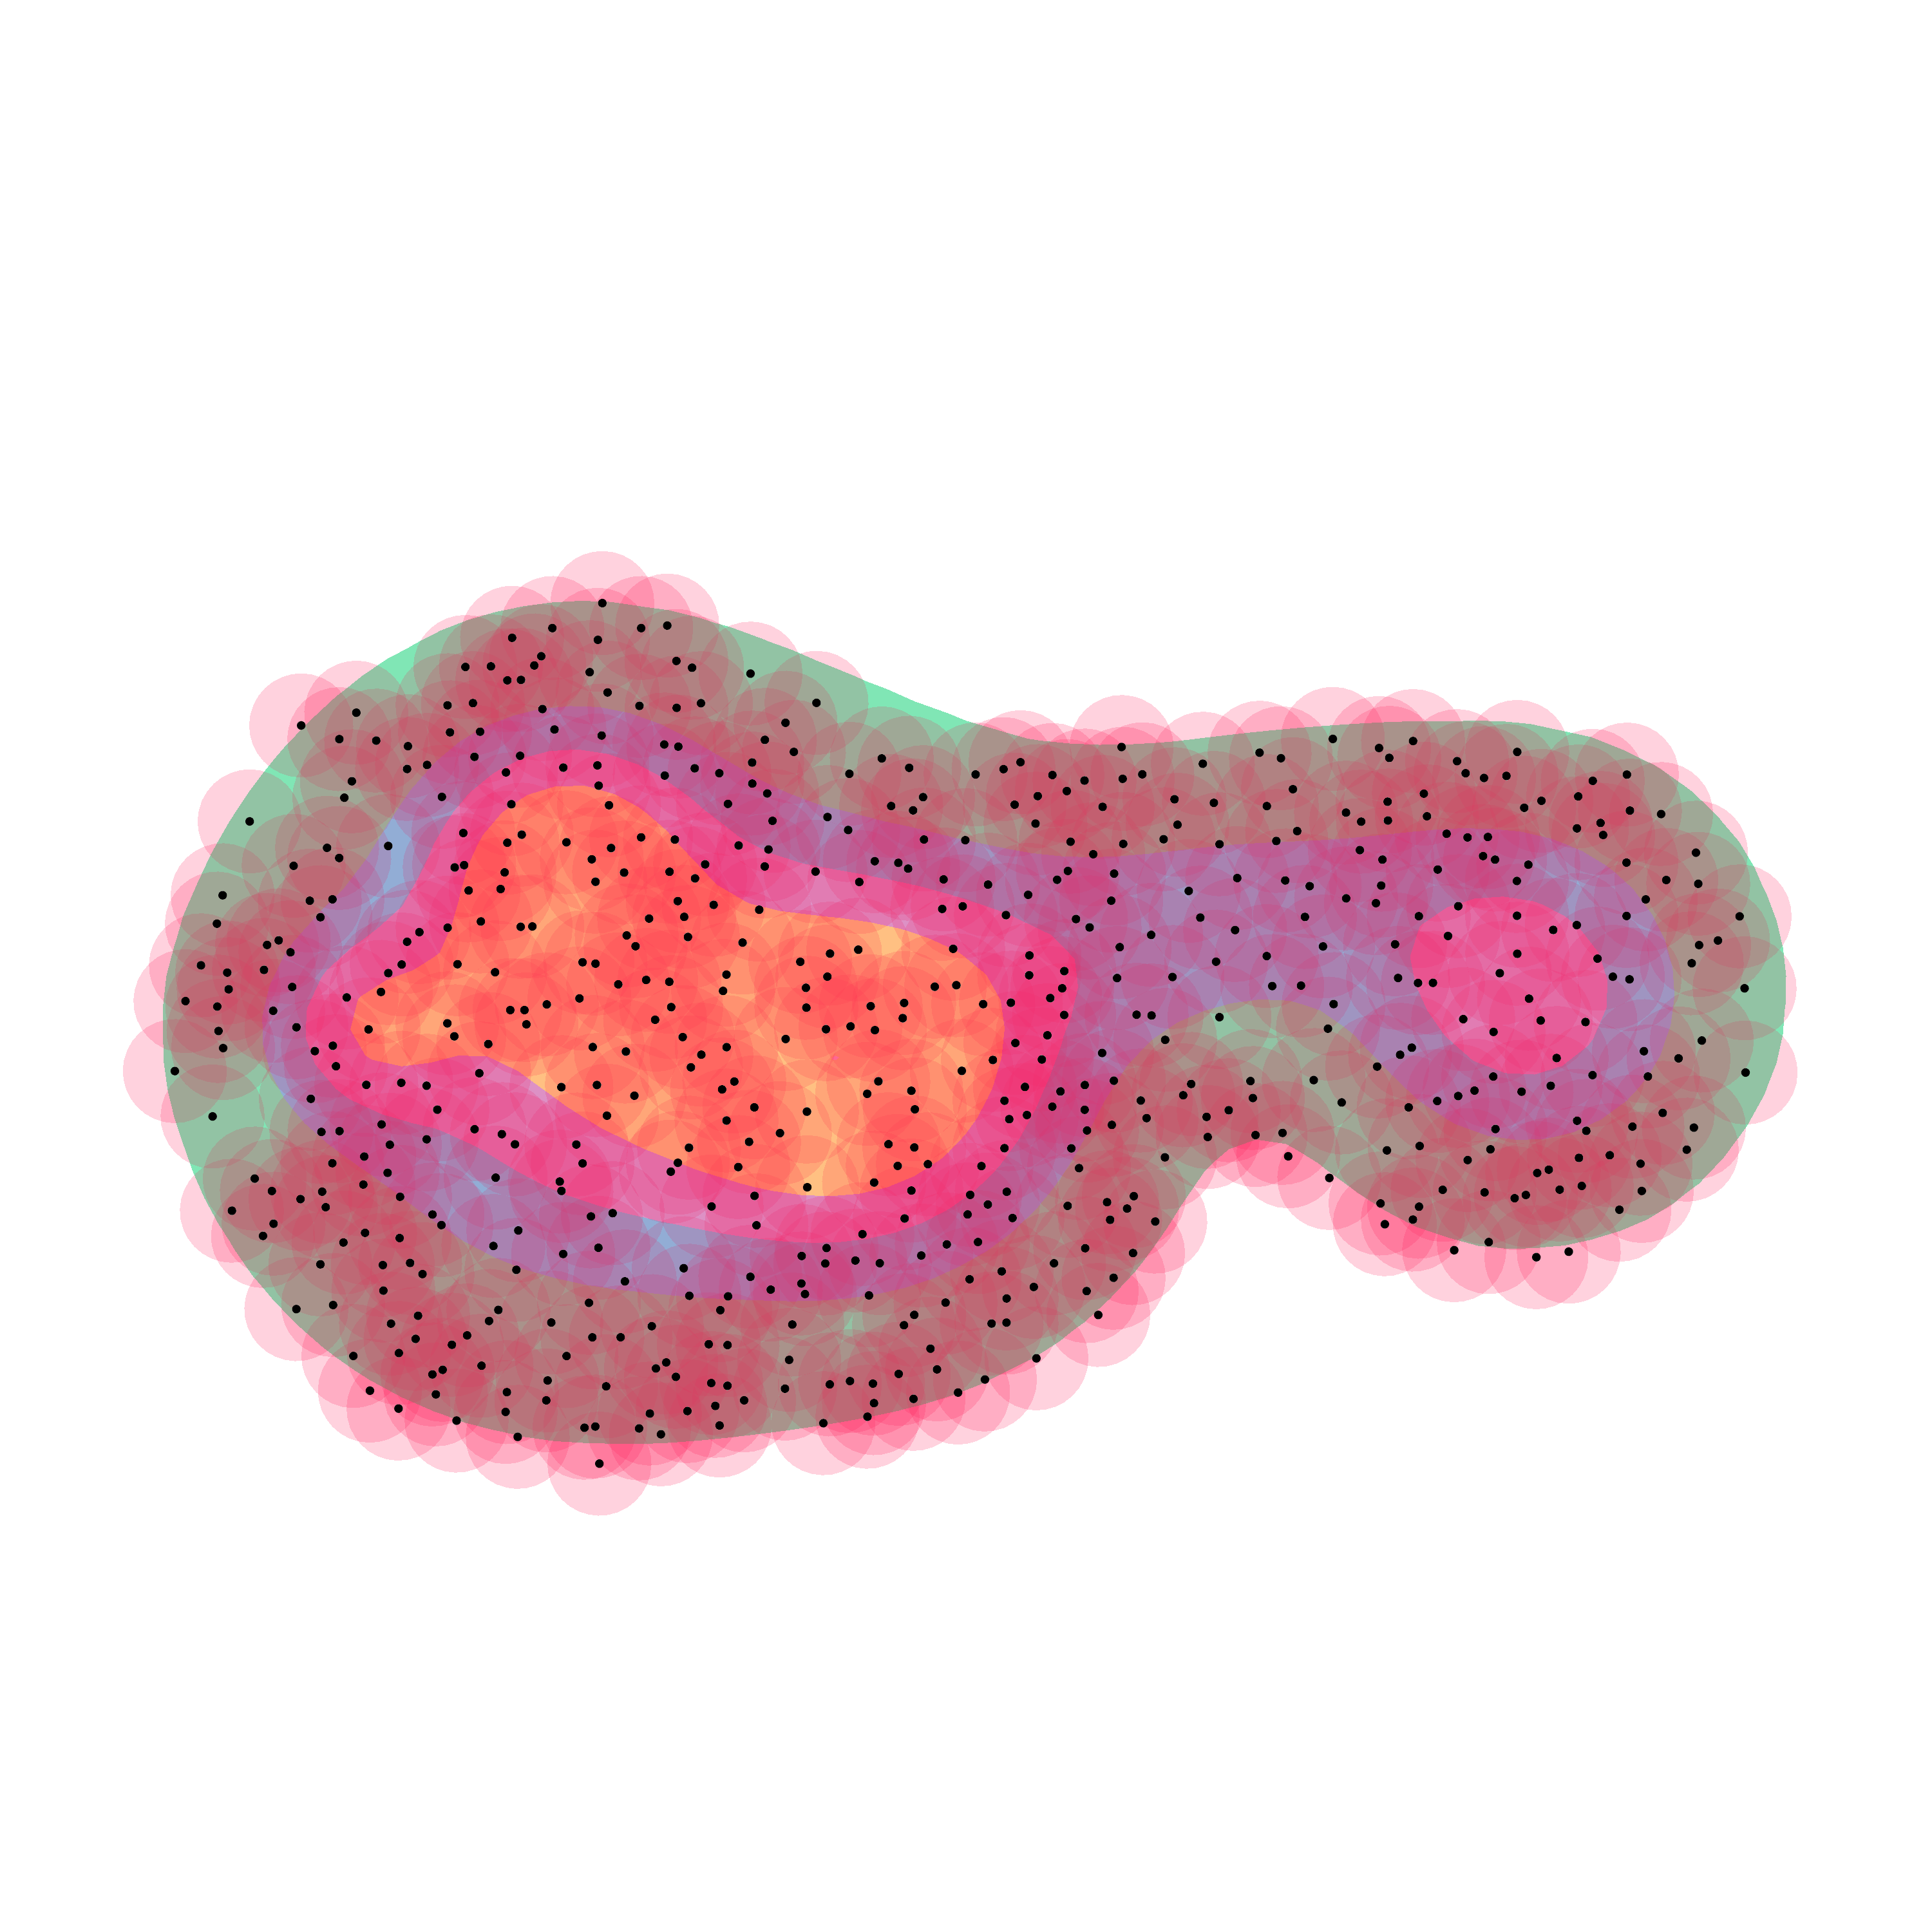
\includegraphics[trim=200 600 200 800, clip, width=0.5\textwidth]{figures/partial3/cover}
  \end{textblock*}
\end{frame}
